%% ut-thesis.tex -- document template for graduate theses at UofT

%% SUMMARY OF FEATURES:
%%
%% All environments, commands, and options provided by the `ut-thesis'
%% class will be described below, at the point where they should appear
%% in the document.  See the file `ut-thesis.cls' for more details.
%%
%% To explicitly set the pagestyle of any blank page inserted with
%% \cleardoublepage, use one of \clearemptydoublepage,
%% \clearplaindoublepage, \clearthesisdoublepage, or
%% \clearstandarddoublepage (to use the style currently in effect).
%%
%% For single-spaced quotes or quotations, use the `longquote' and
%% `longquotation' environments.


%%%%%%%%%%%%         PREAMBLE         %%%%%%%%%%%%

%%  - Default settings format a final copy (single-sided, normal
%%    margins, one-and-a-half-spaced with single-spaced notes).
%%  - For a rough copy (double-sided, normal margins, double-spaced,
%%    with the word "DRAFT" printed at each corner of every page), use
%%    the `draft' option.
%%  - The default global line spacing can be changed with one of the
%%    options `singlespaced', `onehalfspaced', or `doublespaced'.
%%  - Footnotes and marginal notes are all single-spaced by default, but
%%    can be made to have the same spacing as the rest of the document
%%    by using the option `standardspacednotes'.
%%  - The size of the margins can be changed with one of the options:
%%     . `narrowmargins' (1 1/4" left, 3/4" others),
%%     . `normalmargins' (1 1/4" left, 1" others),
%%     . `widemargins' (1 1/4" all),
%%     . `extrawidemargins' (1 1/2" all).
%%  - The pagestyle of "cleared" pages (empty pages inserted in
%%    two-sided documents to put the next page on the right-hand side)
%%    can be set with one of the options `cleardoublepagestyleempty',
%%    `cleardoublepagestyleplain', or `cleardoublepagestylestandard'.
%%  - Any other standard option for the `report' document class can be
%%    used to override the default or draft settings (such as `10pt',
%%    `11pt', `12pt'), and standard LaTeX packages can be used to
%%    further customize the layout and/or formatting of the document.

%% *** Add any desired options. ***
\documentclass{ut-thesis}

%% *** Add \usepackage declarations here. ***
%% The standard packages `geometry' and `setspace' are already loaded by
%% `ut-thesis' -- see their documentation for details of the features
%% they provide.  In particular, you may use the \geometry command here
%% to adjust the margins if none of the ut-thesis options are suitable
%% (see the `geometry' package for details).  You may also use the
%% \setstretch command to set the line spacing to a value other than
%% single, one-and-a-half, or double spaced (see the `setspace' package
%% for details).

\usepackage{titletoc}
\usepackage{amsmath}
\usepackage{amssymb}
\usepackage{graphics}
\usepackage{graphicx}
\usepackage{enumitem}
\graphicspath{{images/}}

\degree{Masters of Science}
\department{Physics}
\gradyear{2016}
\author{Tharshikan Srikannathasan}
\title{Modeling Carbon Monoxide Fields with Artificial Neural Networks}

%% *** NOTE ***
%% Put here all other formatting commands that belong in the preamble.
%% In particular, you should put all of your \newcommand's,
%% \newenvironment's, \newtheorem's, etc. (in other words, all the
%% global definitions that you will need throughout your thesis) in a
%% separate file and use "\input{filename}" to input it here.


%% *** Adjust the following settings as desired. ***

%% List only down to subsections in the table of contents;
%% 0=chapter, 1=section, 2=subsection, 3=subsubsection, etc.
\setcounter{tocdepth}{2}

%% Make each page fill up the entire page.
\flushbottom
%%%%%%%%%%%%      MAIN  DOCUMENT      %%%%%%%%%%%%

\begin{document}

%% This sets the page style and numbering for preliminary sections.
\begin{preliminary}

%% This generates the title page from the information given above.
\maketitle

%% There should be NOTHING between the title page and abstract.
%% However, if your document is two-sided and you want the abstract
%% _not_ to appear on the back of the title page, then uncomment the
%% following line.
%\cleardoublepage

%% This generates the abstract page, with the line spacing adjusted
%% according to SGS guidelines.
\begin{abstract}
Current techniques for inverse modeling carbon monoxide emissions have large biases due to errors in atmospheric transport and tracer gas chemistry in atmospheric models. In addition, current observations used to constrain emissions on regional scales suffer from limited data and low precision measurements. Even with the multiple data stream approach, the covariances between different datasets can be challenging to quantify. A statistical approach offers a means of inverse modeling atmospheric carbon monoxide while avoiding the challenges of model errors We examine the use of a statistical model to simulate atmospheric concentrations of carbon monoxide via feed forward neural networks. This is a a necessary first step toward the use of such networks for the inverse modeling of carbon monoxide emissions. The GEOS-Chem chemical transport model is used to train the network. We show that a maximally connected network with a single hidden layer is sufficient to fit a time series of carbon monoxide concentrations over New York City.
\end{abstract}

%% Anything placed between the abstract and table of contents will
%% appear on a separate page since the abstract ends with \newpage and
%% the table of contents starts with \clearpage.  Use \cleardoublepage
%% for anything that you want to appear on a right-hand page.

%% This generates a "dedication" section, if needed -- just a paragraph
%% formatted flush right (uncomment to have it appear in the document).
%%\begin{dedication}
%%\end{dedication}

%% The `dedication' and `acknowledgements' sections do not create new
%% pages so if you want the two sections to appear on separate pages,
%% uncomment the following line.
%\newpage  % separate pages for dedication and acknowledgements

%% Alternatively, if you leave both on the same page, it is probably a
%% good idea to add a bit of extra vertical space in between the two --
%% for example, as follows (adjust as desired).
%\vspace{.5in}  % vertical space between dedication and acknowledgements

\begin{acknowledgements}
Many thanks to Professor Dylan Jones for teaching a \textbf{dope} introductory class on data assimilation, and for taking me under his supervision. I look forward to our continued collaboration over the length of my doctoral training.
\end{acknowledgements}

%% This generates the Table of Contents (on a separate page).
\tableofcontents
\listoftables
\listoffigures

%% You can add commands here to generate any other material that belongs
%% in the head matter (for example, List of Plates, Index of Symbols, or
%% List of Appendices).

%% End of the preliminary sections: reset page style and numbering.
\end{preliminary}


%%%%%%%%%%%%%%%%%%%%%%%%%%%%%%%%%%%%%%%%%%%%%%%%%%%%%%%%%%%%%%%%%%%%%%%%
%%  Put your Chapters here; the easiest way to do this is to keep     %%
%%  each chapter in a separate file and `\include' all the files.     %%
%%  Each chapter file should start with "\chapter{ChapterName}".      %%
%%  Note that using `\include' instead of `\input' will make each     %%
%%  chapter start on a new page, and allow you to format only parts   %%
%%  of your thesis at a time by using `\includeonly'.                 %%
%%%%%%%%%%%%%%%%%%%%%%%%%%%%%%%%%%%%%%%%%%%%%%%%%%%%%%%%%%%%%%%%%%%%%%%%

\chapter{Introduction}

\section{Carbon Monoxide} \label{intro_CO}
Carbon monoxide (CO) is an odorless, colorless, and toxic gas regulated in Canada. CO is the product of incomplete combustion and a byproduct of hydrocarbon oxidation. It is removed in the atmosphere by reacting with the hydroxide radical OH
%%
\begin{equation}
\text{CO + OH} \rightarrow \text{CO}_2 + \text{H}
\end{equation}
%%
Similar reactions also remove other pollutant gases like methane $(\text{CH}_4)$ and is thus responsible for the oxidative capacity of the atmosphere. Recent data shows that CO concentrations have increased by two to three times the pre-industrial level, largely due to the impact of anthropogenic activity \cite{haan1996}. CO is a known precursor of tropospheric ozone. Therefore, it is vital to understand the dynamics of CO and its sources in order to predict future atmospheric conditions and understand climate change. The lifetime of tropospheric CO is one to two months, long enough to track individual pollution events. CO sources are relatively large compared to other tracer gases. Thus, CO concentrations are easy to detect relative to the background levels. These features render CO a prime candidate for air quality studies.
\section{Sources of CO} \label{intro_COSources}
\cite{duncan2007} calculated the global budget for sources of CO from 1988 to 1997. The results are summarized in Table \ref{table:budget}. 
%%
\begin{table}[!ht]
\centering
\begin{tabular}{|c | c|} 
 \hline
 Source & Emissions \\ [0.5ex] 
 \hline\hline
 Fossil Fuels & 464-487  \\ 
 Bio-fuels & 189 \\
 Biomass Burning & 451-573 \\
 Biogenic NHMC & 354-379 \\
 Methane Oxidation & 778-861 \\ [1ex] 
 \hline
\end{tabular}
\caption{Global budget of CO sources from 1988 to 1997 (Tg/year) \cite{duncan2007}}
\label{table:budget}
\end{table}
\noindent Note that the most important surface sources are from the combustion of fossil fuels, bio-fuels, and biomass. In the troposphere, the oxidation of methane provides the bulk of the background CO concentration. Non-methane hydrocarbons (NHMCs) come from surface vegetation and are a source of CO when oxidized. 

There are large uncertainties with the estimation of regional CO sources. These uncertainties propagate through atmospheric models and lead to sizable errors in the simulation of atmospheric CO fields. \cite{bian2007} used six different models of biomass burning emissions to simulate CO concentrations. The range of the uncertainty in biomass burning was found to be 129 Tg/year. This only accounts for 6$\%$ of the the total CO emissions, but regional emission estimates varied by factors of four or more. The uncertainties resulted in large variability between the various simulations. 
%%%%%%%%%%%%%%%%%%%%%%%%%%%%%%%%%%%%%%%%%%%%%%%%%%%%%%%%%%%%%%%%%%%%%%%%%%%%%%%
\begin{figure*}
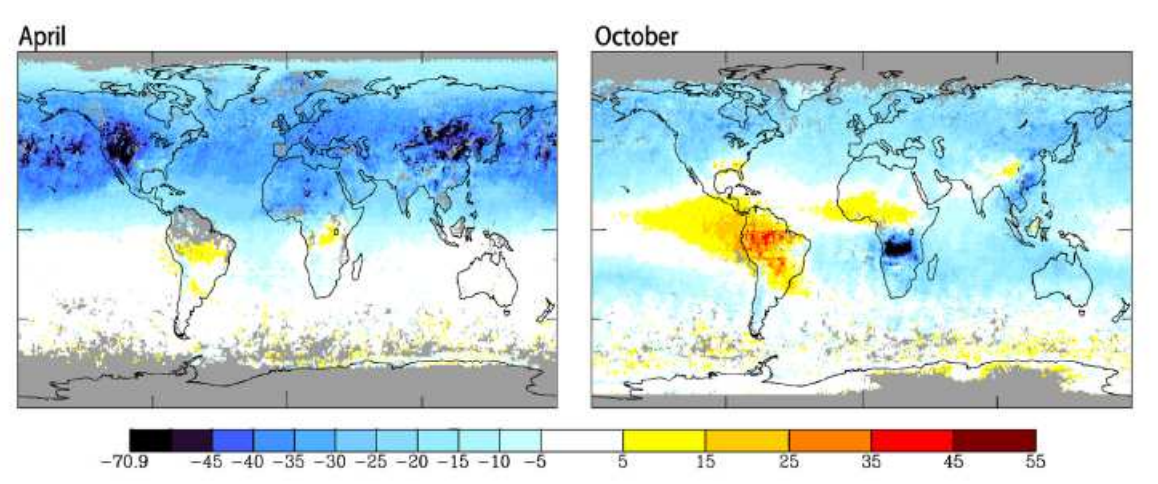
\includegraphics[width=\linewidth]{shindell2007plot}
\caption{Differences between the chemical transport multi-model mean CO and MOPITT V3 CO for 2000-2004 (ppbv) at 500 hPa. The background CO field is 200 ppbv. Plot from \cite{shindell2006}.}
\label{fig:shindell2007plot}
\end{figure*}
%
Another study, conducted by \cite{shindell2006} compared 26 different chemical transport models (CTMs) and found that they successfully reproduced the large scale spatial and temporal features of CO. However, the study also revealed significant biases between modeled and observed CO (See Figure \ref{fig:shindell2007plot}). Note that the average CO concentration is underestimated in the northern hemisphere during April and over the biomass burning regions of Africa during October. It turns out that CO concentrations are consistently underestimated in the northern hemisphere throughout the year \cite{shindell2006}. This is due to the underestimation of CO surface emissions caused by anthropogenic activity. Furthermore, the variability between the individual models was large even when the mean agreed with the observations. Again, this is due to incorrect estimations of emissions from NHMCs and gas oxidation. The study also found that transport was not as important as differences in NHMC estimates. \cite{liu2010} used the GEO-Chem CTM to analyze CO variation over tropical latitudes. The results were compared to the Microwave Limb Sounder (MLS) and Tropospheric Emission Satellite (TES) retrievals of CO. Again, spatial and seasonal CO variability was captured but there were underestimations in the biomass burning in the southern latitudes. The study also showed a temporal displacement in CO seasonal maxima in the troposphere over South America. The findings were linked to erroneous vertical transport and NHMC sources. Another study was conducted by \cite{ott2011}) concerning the influence of convective transport on CO fields. They perturbed the GEOS-5 convective parameters in an ensemble of eight simulations. The parameter changes caused large variability on CO concentrations over Africa, Indonesia, and South America. These areas notably feature significant biomass burning and convection in the lower atmosphere. The aforementioned results point to similar issues with modeling CO distribution: uncertainties in source estimates and in the transport. It is clear that one must better constrain estimates of CO sources to increase the accuracy of the CO simulations that rely on them.
\subsection{Estimation of CO Sources}
\label{sec:estimating co}
%

The two most common methods of calculating CO emissions are referred to as the bottom-up, and top-down approaches. The former method relies on regional and international energy statistics for estimates of both fossil fuel and biofuel sources. This data is combined with  geo-information such as population statistics, road type, and land cover data to approximate anthropogenic sources of CO. However, these data are often extrapolated in space and time. For example, statistics from countries with limited data are replaced with information from western countries \cite{streets2003}. For biomass burning, satellite observations are combined with ecosystem types to produce CO emission estimates. Despite this, it is still difficult to constrain burned area and fuel loads. \cite{van2010} showed that biomass burning calculations are uncertain to a minimum of 20$\%$.

The top-down approach uses ideas from the field of inverse modeling. This method attempts to minimize the differences between CTM simulations and observed CO concentrations by adjusting sources of CO. Most studies have used low-resolution Bayesian methods. That is, emissions are grouped by region and continent. Emissions are then scaled with respect to each unit to minimize the residual error between the model and the observations. However, this process leads to aggregation errors which have been shown to significantly impact emission estimates \cite{jiang2011}. Another top down approach considers techniques that fall under variational methods. Four dimensional variational data assimilation (4D-Var) is one such technique. 4D Var uses so called adjoint methods, which have the advantage of allowing emission estimates to be made at the native resolution of the CTM. These methods have immediate problems concerning data resolution limits in both the spatial and temporal domain. Aircraft and surface based observations don't guarantee a well constrained estimate on CO sources. \cite{jones2009} used CO retreivals from TES and MOPITT to constrain sources using the GEOS-Chem CTM. They found that differences in \textit{a posteriori} emission estimates were roughly 20$\%$ of the \textit{a priori} source information.

\section{Objective of Manuscript}
\label{sec:scope}

To summarize the previous sections, it is apparent that model biases are a challenge for the inverse modeling of CO emissions. Both satellite and surface CO data streams are insufficient to quantify emissions on regional subscales. Combining datasets is one solutions of overcoming the data sparsity problems. However, calculating covariances between the different streams of data can prove to be challenging. In this manuscript we use statistical methods to model CO fields. These methods avoid calculating model biases and covariances. This allows combinations of multivariate data to be included in the modeling of CO concentrations. It will also circumvent the challenges associated with model biases. This gain comes at the cost of losing information about the structure of the model. In particular, the free parameters of statistical models are often difficult to interpret outside of a handful of toy models. Our long term goal is to use a statitical approach to estimate CO sources. As a first step, the work presented in this report is focused on predicting CO concentrations using neural networks. If we can successfully predict CO fields then that information will lead to better estimates of CO sources.

First, the reader will be introduced to notion of artificial neural networks. The notion of training a neural network will be discussed, along with a derivation of the back-propagation algorithm. The network will applied to a nonlinear univariate regression problem. Then we attempt to model a Lorentz dynamical system using a neural network generator and discuss some limitations of FFNNs. Finally, we train the network on the GEOS-Chem chemical transport model to predict yearly CO fields.
\chapter{Artificial Neural Networks}
\section{What is a Neural Network?}
\label{sec: nn_intro}

In the field of biology, a \textit{neuron} is a cell that processes information by way of electrical and chemical stimulation. These cells are at the core of nature's computing architecture, the nervous system. Neurons are made up of a soma, axons, and dendrites. The soma is the body of the neuron while signals are captured by dendrites and transmitted through the axons. When a neuron receives a signal, it will output a response if the input is higher than some internal threshold. A mesh of many of these neurons is called a neural network. The human brain has an estimated 100 billion such neurons interconnected in complex networks. It is believed the dense computing power of the brain is a direct result of this topology. In statistics and machine learning, an \textit{artificial neural network} (ANN) is a network of computing units loosely inspired by the aforementioned systems seen in biology. ANNs are used to approximate functions and classify patterns. An artificial neuron is a simple computing node that takes in a signal \textit{s} and fires according to an internal activation rule

\begin{equation*}
n(s) = \begin{cases} 1 &\mbox{if } s \geq t \\ 
0&\mbox{if } s < t \end{cases}
\end{equation*}

\noindent where \textit{t} is the threshold of the neuron. The signal comes from the outputs of other neurons

\begin{align*}
s & = w_1x_1 + w_2x_2 + ... + w_Nx_N \\
& = \textbf{x}^T\textbf{w}
\end{align*}

\noindent where $\textbf{x}^T\textbf{w}$ is the euclidean inner product between a vector of weights \textbf{w} and a vector of inputs \textbf{x}. In this language the neuron can be defined as

\begin{equation}
n(z) = \begin{cases} 1 &\mbox{if } z \geq 0 \\ 
0&\mbox{if } z < 0 \end{cases} \quad \mbox{where } z = \textbf{x}^T\textbf{w} + b
\end{equation}

\begin{figure}
\centering
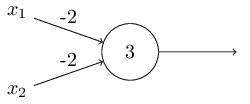
\includegraphics[width=0.4\textwidth]{simple_neuron}
\caption{A single neuron NAND gate with two identical weights, $w_1 = w_2 = -2$ and a bias $b = 3$}
\label{fig:simple_neuron}
\end{figure}

\noindent where \textit{b} is the so called bias of the neuron. With this definition, one can pick weights such that the neuron can model a NAND gate. Recall that a NAND gate is an inverted AND gate. Therefore we wish to take two inputs A and B and output NOT(A and B). Consider a neuron that takes two binary inputs $(x_1,x_2)$ and outputs a binary response according to the architecture in Figure \ref{fig:simple_neuron}. In this simple case, the weights and bias are trivial to choose. For example, if $(x_1,x_2)=(1,0)$ then we have

\begin{align*}
n\left(w_1x_1 + w_2x_2 + b\right) & = n\Big((-2)(1) + (-2)(0) + 3\Big) \\
& = n(1) \\
& = 1
\end{align*}

\noindent The other permutations of inputs clearly describe the properties of the function we wished to recreate. The natural question to ask is one of generality, how does a step function model complex time series data or classify animals in images? The answer lies in the organization of  many neurons and the resulting topology that is formed from the grouping.

\section{Architectures, Activation, and Assimilation}
\label{sec: three_As}

The \textit{architecture} of a neural network refers to the structure that exists between individual nodes of a network. This paper will be discussing \textit{feed-forward neural networks} (FFNNs). A FFNN consists of \textit{L} layers of neurons with each layer containing $n_l$ single neurons, where $l=1, 2, ..., L$. The first layer of neurons are called the input layer. This layer is unique in the sense that it does not compute, but only sends the initial information into the network. From this point, the information is sent from one layer to the next and each neuron in a succeeding layer will fire according to it's activation function and input signal from the preceding layer of neurons.

\begin{figure}[!htb]
\centering
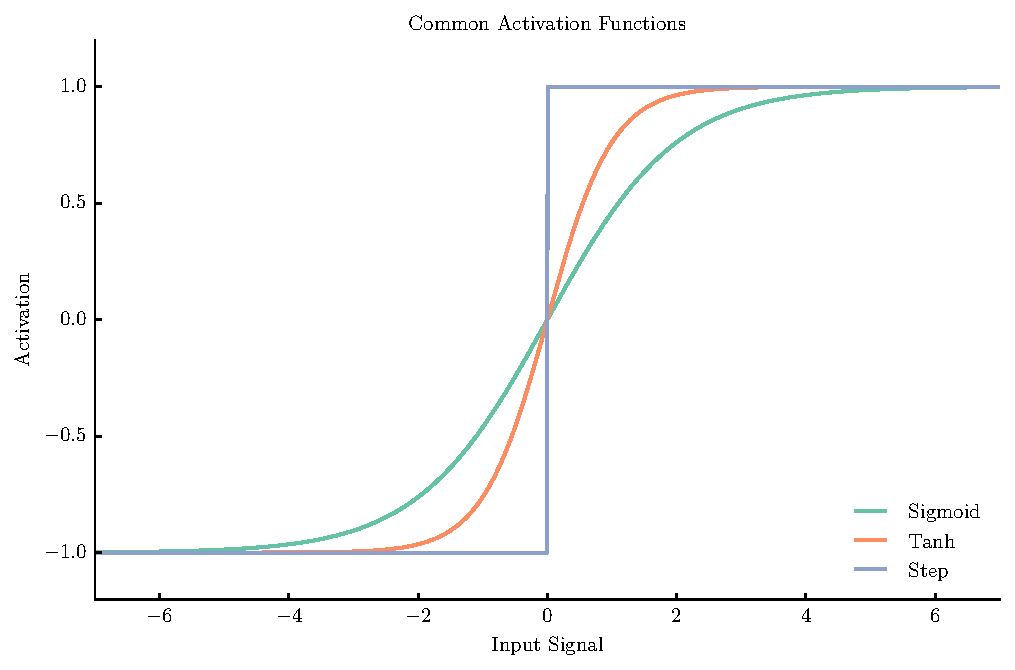
\includegraphics[width=\textwidth]{activation_functions.pdf}
\caption{Three common activation functions used in neural networks.}
\label{fig:act_fun}
\end{figure}

The \textit{activation function} of a FFNN refers to a non-linearity $\phi(\cdot)$ that is applied after the node receives a signal. For practical purposes, a smooth approximation to the step function is preferred. Hence $\phi$ is usually some sort of sigmodial function such as the logistic function or the tanh function (Figure \ref{fig:act_fun}). These functions have convenient analytic properties that one can take advantage of to train the network. The last layer of the network is called the output layer. This layer takes the signal from the last layer of hidden neurons and sends the signal through a final transfer function, which translates the output of the network to a result that can be understood within the context of the problem. Such transfer functions include an identity mapping (for regression) or a soft-max mapping for multi-label classification. FFNN neurons are all maximally connected. This means that every neuron in layer \textit{l} is connected to the neurons in layers $l - 1$ and $l + 1$. The network from Figure \ref{fig:simple_neuron} can be considered a FFNN with 0 hidden layers, 2 input neurons and 1 output neuron. More generally, the strength of connectivity between neuron \textit{j} in layer $l-1$ and neuron \textit{k} in layer $l$ is denoted by the weight $w^{l}_{jk}$ and neuron \textit{j} in layer \textit{l} carries a bias of $b^{l}_j$. One of the most interesting aspects of FFNNs is the ability to compute \textit{\textbf{any}} function with a single hidden layer of neurons. That is, given any function $f$ there exists a FFNN that can closely approximate \textit{f}. This is stated formally as the \textbf{Universal Approximation Theorem} (UAT).
%%%%%%%%%%%%%%%%%%%%%%%%%%%%%%%%%%%%%%%%%%%%%%%%%%%%%%%%%%%%%%%%%%%%%%%%%%%%%%%
\subsection{The Universal Approximation Theorem}
%%%%%%%%%%%%%%%%%%%%%%%%%%%%%%%%%%%%%%%%%%%%%%%%%%%%%%%%%%%%%%%%%%%%%%%%%%%%%%%
Let $g(\cdot)$ be a non-constant, bounded, and monotonically-increasing continuous function. Let $I_m$ denote the \textit{m}-dimensional unit hypercube $[0, 1]^m$. The space of continuous functions on $I_m$ is denoted by $C(I_m)$. Then, given any function $f\,\epsilon\,C(I_m)$ and $\epsilon > 0$, there exists an integer $n$, real constants $\alpha_i$, $\beta_i\,\epsilon\,\mathbb{R}$ and real vectors $\boldsymbol{\omega}_i \,\epsilon\,\mathbb{R}^m$, where $i=1,...,n$, such that we may define
%%%%%%%%%%%%%%%%%%%%%%%%%%%%%%%%%%%%%%%%%%%%%%%%%%%%%%%%%%%%%%%%%%%%%%%%%%%%%%%
\begin{equation*}
F(\textbf{x}) = \sum_{i=1}^{n} \alpha_i\,g(\boldsymbol{\omega}^T_i\textbf{x} + \beta_i)
\end{equation*}
%%%%%%%%%%%%%%%%%%%%%%%%%%%%%%%%%%%%%%%%%%%%%%%%%%%%%%%%%%%%%%%%%%%%%%%%%%%%%%%
as an approximate realization of the function \textit{f} where \textit{f} is independent of $g_i$; that is,
%%%%%%%%%%%%%%%%%%%%%%%%%%%%%%%%%%%%%%%%%%%%%%%%%%%%%%%%%%%%%%%%%%%%%%%%%%%%%%%
\begin{equation*}
|F(x) - f(x)| < \epsilon
\end{equation*}
%%%%%%%%%%%%%%%%%%%%%%%%%%%%%%%%%%%%%%%%%%%%%%%%%%%%%%%%%%%%%%%%%%%%%%%%%%%%%%%
for all $x\,\epsilon\,I_m$. In other words, functions of the form $F(x)$ are dense in $C(I_m)$. Furthermore, this theorem still holds when replacing $I_m$ with any compact subset of $\mathbb{R}^m$. 

While the \textit{rigorous} proof of the UAT is far beyond the scope of this manuscript, the following discussion will sketch how the UAT connects to FFNNs. Consider a FFNN with a single hidden layer with \textit{n} hidden neurons. For simplicity let the input be two dimensional and the output one dimensional. Let us denote these variables as $\textbf{x}=(x_1, x_2)$, and $y$. The first step to computing the signals $z_i$ into the hidden layer of neurons, where $i=1,2,...,n$
%%%%%%%%%%%%%%%%%%%%%%%%%%%%%%%%%%%%%%%%%%%%%%%%%%%%%%%%%%%%%%%%%%%%%%%%%%%%%%%
\begin{align*}
z_1 & = w^2_{11}x_1 + w^2_{21}x_2 + b^2_1 \\
z_2 & = w^2_{12}x_1 + w^2_{22}x_2 + b^2_2 \\
\vdots{}  \\
z_n & = w^2_{1n}x_1 + w^2_{2n}x_2 + b^2_n \\
\end{align*}
%%%%%%%%%%%%%%%%%%%%%%%%%%%%%%%%%%%%%%%%%%%%%%%%%%%%%%%%%%%%%%%%%%%%%%%%%%%%%%%
The hidden layer has a continuous output $a_i=\phi(z_i)$, where $\phi$ is a sigmoidal non-linearity. These activations are sent from the hidden layer to the output layer via the 2nd set of weights. Here, the final non-linearity is applied to give the output \textit{y}
%%%%%%%%%%%%%%%%%%%%%%%%%%%%%%%%%%%%%%%%%%%%%%%%%%%%%%%%%%%%%%%%%%%%%%%%%%%%%%%
\begin{equation*}
y = \psi\left(w^3_{11}a_1 + w^3_{21}a_2 + ... + w^3_{n1}a_n\right)
\end{equation*}
%%%%%%%%%%%%%%%%%%%%%%%%%%%%%%%%%%%%%%%%%%%%%%%%%%%%%%%%%%%%%%%%%%%%%%%%%%%%%%%
If $\psi$ is the identity mapping\footnote{This holds for all $\psi$, not just linear functions}, then we have exactly the construction of a function as shown in the UAT
%%%%%%%%%%%%%%%%%%%%%%%%%%%%%%%%%%%%%%%%%%%%%%%%%%%%%%%%%%%%%%%%%%%%%%%%%%%%%%%
\begin{align}
y & = w^3_{11}\phi({\textbf{w}^2_1}^T\textbf{x} + b^2_1) + ... + w^3_{n1}\phi({\textbf{w}^2_n}^T \textbf{x}+ b^2_n) \nonumber \\
& = \sum_{i=1}^{n} w^3_{i1}\phi({\textbf{w}^2_i}^T \textbf{x}+ b^2_i)
\end{align}
%%%%%%%%%%%%%%%%%%%%%%%%%%%%%%%%%%%%%%%%%%%%%%%%%%%%%%%%%%%%%%%%%%%%%%%%%%%%%%%
Therefore by the UAT the construction above will approximate any one dimensional function $f \, \in \, \mathbb{R}$.
%%%%%%%%%%%%%%%%%%%%%%%%%%%%%%%%%%%%%%%%%%%%%%%%%%%%%%%%%%%%%%%%%%%%%%%%%%%%%%%

The astute reader might be left with more questions at the end of the preceding analysis. How many hidden neurons does it take to approximate a function? How does one choose the weights and biases such that the approximation is a \textit{good} one? While the UAT guarantees the existence of such a network, little is claimed about how to go about constructing the architecture. The problem of choosing parameters becomes intractable as the number of hidden neurons increases. 

In a FFNN of one dimensional inputs and outputs, the number of adjustable parameters is given by $N_p=3n$, where \textit{n} is the number of hidden neurons in a single hidden layer. \textit{Deep neural networks} are often used to classify images. In the problem of digit classification, a network ingests an input image of size 28x28 which means the input space is 784 dimensional. The output space is 10 dimensional which corresponds to the 10 possible digits that can be recognized. Suppose further that a four layer FFNN is used to solve this problem. Even if there are only 10 neurons in each hidden layer, that corresponds to over 8000 adjustable weights and biases. Thus, in order to proceed we must consider an algorithmic way of optimizing these values to produce the \textit{best} network possible. This is referred to as the \textit{learning problem} in machine learning and it brings us to the final aspect of ANNs, assimilation.

\section{The Learning Problem} \label{learning_problem}

Suppose we are given a set of training examples $S=\lbrace(\textbf{x}_i, \textbf{y}_i), i=1,2,...,N| (\textbf{x}_i, \textbf{y}_i)\, \epsilon \, \mathbb{R}^{d_x} \times \mathbb{R}^{d_y}\rbrace$. The goal is to construct an \textit{L} layer FFNN that takes $\textbf{x}_i$ as an input and outputs an estimate $\boldsymbol{\eta}_i(\Theta)=\boldsymbol{\eta}(\textbf{x}_i| \Theta)$, where $\Theta=\lbrace \textbf{W}, \textbf{b} \rbrace$ is the set of weights and biases describing the network. We seek a parameter set $\Theta=\Theta^*$ such that $\boldsymbol{\eta}_i(\Theta^*)\approx\textbf{y}_i$. Since $\Theta$ is a random variable, $\Theta^*$ must be correspond to the parameter set that is most likely to be observed given what is known about the training data. We construct this probability distribution under the following assumptions. Assume each $\boldsymbol{\eta}_i$ is independent and identically distributed (i.i.d) and normally distributed around the target $\textbf{y}_i$. Furthermore, we constrain the weights to be normally distributed around \textbf{0} to avoid over-fitting of the training data and all biases are assumed to be drawn from a uniform distribution over some subset of the real line. Bayes Theorem can now be invoked to calculate the posterior distribution of $\Theta$ given the training examples
%%%%%%%%%%%%%%%%%%%%%%%%%%%%%%%%%%%%%%%%%%%%%%%%%%%%%%%%%%%%%%%%%%%%%%%%%%%%%%%
\begin{equation}
P(\Theta|S) = \frac{P(S|\Theta)P(\Theta)}{\int P(S|\Theta)P(\Theta) d\Theta}
\end{equation}
%%%%%%%%%%%%%%%%%%%%%%%%%%%%%%%%%%%%%%%%%%%%%%%%%%%%%%%%%%%%%%%%%%%%%%%%%%%%%%%
Maximizing this function is equivalent to minimizing $-ln\left[P(\Theta|S)\right]$. If we discard additive constants, the problem of maximizing $P(\Theta|S)$ transforms into the problem of minimizing the so called \textit{cost function}
%%%%%%%%%%%%%%%%%%%%%%%%%%%%%%%%%%%%%%%%%%%%%%%%%%%%%%%%%%%%%%%%%%%%%%%%%%%%%%%
\begin{equation}
E(\Theta|\textbf{X}) = \frac{1}{2N} \left[\boldsymbol{\eta}(\textbf{X}|\Theta) - \textbf{Y}\right] {\left[\boldsymbol{\eta}(\textbf{X}|\Theta) - \textbf{Y}\right]}^T \nonumber + \frac{\lambda}{2N_w}\sum_{l} \textbf{W}_l \textbf{W}_l^T
\label{cost_cost}
\end{equation}
%%%%%%%%%%%%%%%%%%%%%%%%%%%%%%%%%%%%%%%%%%%%%%%%%%%%%%%%%%%%%%%%%%%%%%%%%%%%%%%
The notation has been vectorized for brevity. \textbf{X} is the $N \times d_x$ input data matrix and \textbf{Y} is the $N \times d_y$ target data matrix. $\boldsymbol{\eta}(\textbf{X})$ is the output of the network, $N_w$ is the total number of weights, $\lambda$ is the regularization hyper-parameter, and $\textbf{W}_l$ are the matrix of weights connecting layers $l-1$ and $l$ such that each element of $\textbf{W}_l$ is $w^l_{jk}$. Now that we have a well defined objective in the learning problem, we discuss the algorithms used to find $\Theta^*$.
%%%%%%%%%%%%%%%%%%%%%%%%%%%%%%%%%%%%%%%%%%%%%%%%%%%%%%%%%%%%%%%%%%%%%%%%%%%%%%%
\subsection{Minimizing $E(\Theta)$}

In order to computationally minimize $E(\Theta)$ it is necessary to know the gradient of the cost with respect to all elements of $\Theta$. The \textit{back-propagation algorithm}, published in 1986 by \cite{rumelhart1988l} describes an algorithmic procedure for computing the gradient of the cost function. Note that for our network from section \ref{learning_problem} we have $\Theta=\lbrace \textbf{W}_2, \textbf{W}_3, ..., \textbf{W}_L, \textbf{b}_2, ..., \textbf{b}_{L} \rbrace$. Let us denote the inputs and outputs to layer $l$ as $\textbf{z}_l$ and $\textbf{a}_l$ respectively. The signals are related through the activation function\footnote{Note that the sum between the weighted components and the bias is broadcast row-wise.}
%%%%%%%%%%%%%%%%%%%%%%%%%%%%%%%%%%%%%%%%%%%%%%%%%%%%%%%%%%%%%%%%%%%%%%%%%%%%%%%
\begin{equation}
\textbf{a}_l = \psi(\textbf{z}_l), \, \textbf{z}_l = \textbf{a}_{l - 1}\textbf{W}_l + \textbf{b}_l
\end{equation}
%%%%%%%%%%%%%%%%%%%%%%%%%%%%%%%%%%%%%%%%%%%%%%%%%%%%%%%%%%%%%%%%%%%%%%%%%%%%%%%
Note that $\textbf{z}_1$ does not exist, as there is no signal going into layer 1, $\textbf{a}_L = \boldsymbol{\eta}(\textbf{X})$\footnote{The $\Theta$ has been suppressed here for brevity.}, and $\textbf{a}_1 = \textbf{X}$. The recursive structure of the network implies that derivatives in layer $l$ depend on layers \textit{ahead} of them. To see this note that for $l=L$ we have
%%%%%%%%%%%%%%%%%%%%%%%%%%%%%%%%%%%%%%%%%%%%%%%%%%%%%%%%%%%%%%%%%%%%%%%%%%%%%%%
\begin{equation*}
\frac{\partial E}{\partial \textbf{W}_L} = 
\frac{1}{N} \textbf{a}^T_{L - 1}
\left[\boldsymbol{\eta}(\textbf{X}) - \textbf{Y}\right] \odot
\psi^{\prime}(\textbf{z}_{L}) + \frac{\lambda}{N_w}\textbf{W}_L
\end{equation*}
%%%%%%%%%%%%%%%%%%%%%%%%%%%%%%%%%%%%%%%%%%%%%%%%%%%%%%%%%%%%%%%%%%%%%%%%%%%%%%%
\begin{equation*}
\frac{\partial E}{\partial \textbf{b}_L} = 
\frac{1}{N} \textbf{1}^T
\left[\boldsymbol{\eta}(\textbf{X}) - \textbf{Y}\right] \odot
\psi^{\prime}(\textbf{z}_{L})
\end{equation*}
%%%%%%%%%%%%%%%%%%%%%%%%%%%%%%%%%%%%%%%%%%%%%%%%%%%%%%%%%%%%%%%%%%%%%%%%%%%%%%%
Where $\odot$ represents the element-wise product, $\psi^{\prime}(\cdot)$ is the derivative of the transfer function applied element-wise, and \textbf{1} is a vector of 1's. Defining $\boldsymbol{\delta}_{L} = \frac{1}{N} \left[\boldsymbol{\eta}(\textbf{X}) - \textbf{Y}\right] \odot \psi^{\prime}(\textbf{z}_{L})$ we have
%%%%%%%%%%%%%%%%%%%%%%%%%%%%%%%%%%%%%%%%%%%%%%%%%%%%%%%%%%%%%%%%%%%%%%%%%%%%%%%
\begin{equation*}
\frac{\partial E}{\partial \textbf{W}_L} = 
\textbf{a}^T_{L - 1}\boldsymbol{\delta}_{L} + \frac{\lambda}{N_w}\textbf{W}_L
\end{equation*}
%%%%%%%%%%%%%%%%%%%%%%%%%%%%%%%%%%%%%%%%%%%%%%%%%%%%%%%%%%%%%%%%%%%%%%%%%%%%%%%
\begin{equation*}
\frac{\partial E}{\partial \textbf{b}_L} = 
\textbf{1}^T\boldsymbol{\delta}_{L}
\end{equation*}
%%%%%%%%%%%%%%%%%%%%%%%%%%%%%%%%%%%%%%%%%%%%%%%%%%%%%%%%%%%%%%%%%%%%%%%%%%%%%%%
A pattern reveals itself as we consider $l=L-1$
%%%%%%%%%%%%%%%%%%%%%%%%%%%%%%%%%%%%%%%%%%%%%%%%%%%%%%%%%%%%%%%%%%%%%%%%%%%%%%%
\begin{eqnarray*}
\frac{\partial E}{\partial \textbf{W}_{L - 1}} & = & 
\frac{1}{N} \textbf{a}^T_{L - 2}
\boldsymbol{\delta}_L \textbf{W}^T_L \odot
\psi^{\prime}(\textbf{z}_{L - 1}) + \frac{\lambda}{N_w}\textbf{W}_{L - 1} \nonumber \\
& = & \textbf{a}^T_{L - 2}
\boldsymbol{\delta}_{L - 1} + \frac{\lambda}{N_w}\textbf{W}_{L - 1}
\end{eqnarray*}
%%%%%%%%%%%%%%%%%%%%%%%%%%%%%%%%%%%%%%%%%%%%%%%%%%%%%%%%%%%%%%%%%%%%%%%%%%%%%%%
\begin{eqnarray*}
\frac{\partial E}{\partial \textbf{b}_{L - 1}} & = & 
\frac{1}{N} \textbf{1}^T
\boldsymbol{\delta}_L \textbf{W}^T_L \odot
\psi^{\prime}(\textbf{z}_{L - 1}) \nonumber \\
& = & \textbf{1}^T
\boldsymbol{\delta}_{L - 1}
\end{eqnarray*}
%%%%%%%%%%%%%%%%%%%%%%%%%%%%%%%%%%%%%%%%%%%%%%%%%%%%%%%%%%%%%%%%%%%%%%%%%%%%%%%
where $\boldsymbol{\delta}_{L - 1} = \frac{1}{N} \boldsymbol{\delta}_L \textbf{W}^T_L \odot \psi^{\prime}(\textbf{z}_{L - 1})$. This is extended by induction until $l = 2$ and we have the complete gradient of the cost function
%%%%%%%%%%%%%%%%%%%%%%%%%%%%%%%%%%%%%%%%%%%%%%%%%%%%%%%%%%%%%%%%%%%%%%%%%%%%%%%
\begin{equation}
\boldsymbol{\delta}_{l} = \frac{1}{N} \boldsymbol{\delta}_{l + 1} \textbf{W}^T_{l + 1} \odot \psi^{\prime}(\textbf{z}_{l})
\end{equation}
%%%%%%%%%%%%%%%%%%%%%%%%%%%%%%%%%%%%%%%%%%%%%%%%%%%%%%%%%%%%%%%%%%%%%%%%%%%%%%%
\begin{equation}
\frac{\partial E}{\partial \textbf{W}_{l}} = 
\textbf{a}^T_{l - 1}
\boldsymbol{\delta}_{l} + \frac{\lambda}{N_w}\textbf{W}_{l}
\end{equation}
%%%%%%%%%%%%%%%%%%%%%%%%%%%%%%%%%%%%%%%%%%%%%%%%%%%%%%%%%%%%%%%%%%%%%%%%%%%%%%%
\begin{equation}
\frac{\partial E}{\partial \textbf{b}_{l}} = \textbf{1}^T
\boldsymbol{\delta}_{l}
\end{equation}
%%%%%%%%%%%%%%%%%%%%%%%%%%%%%%%%%%%%%%%%%%%%%%%%%%%%%%%%%%%%%%%%%%%%%%%%%%%%%%%
Notice that $\boldsymbol{\delta}_l$ can be cast as a derivative of the cost with respect to the signal input to layer $l$, $\partial E/ \partial \textbf{z}_{l}$. Therefore, one can consider $\boldsymbol{\delta}_{l}$ as being a measure of the error in layer $l$ of the network. With this result, the back-propagation algorithm can be stated in its entirety.
%%%%%%%%%%%%%%%%%%%%%%%%%%%%%%%%%%%%%%%%%%%%%%%%%%%%%%%%%%%%%%%%%%%%%%%%%%%%%%%
\subsection{The Back-propagation Algorithm}
\label{backprop}
%%%%%%%%%%%%%%%%%%%%%%%%%%%%%%%%%%%%%%%%%%%%%%%%%%%%%%%%%%%%%%%%%%%%%%%%%%%%%%%
\begin{enumerate}[topsep=0pt,itemsep=0ex,partopsep=1ex,parsep=1ex]
\item Set $\textbf{a}_1 = \textbf{X}$
\item Compute $\textbf{z}_l = \textbf{a}_{l - 1}\textbf{W}_l + \textbf{b}_l$ and $\textbf{a}_l = \psi(\textbf{z}_l)$ for $l=2,3,...,L$
\item Compute $\boldsymbol{\delta}_L = \frac{1}{N} \left[\boldsymbol{\eta}(\textbf{X}) - \textbf{Y}\right] \odot \psi^{\prime}(\textbf{z}_{L})$
\item Compute $\boldsymbol{\delta}_{l} = \frac{1}{N} \boldsymbol{\delta}_{l + 1} \textbf{W}^T_{l + 1} \odot \psi^{\prime}(\textbf{z}_{l})$ for $l=L - 1, L - 2, ...., 2$
\item $\nabla E(\textbf{W}, \textbf{b})$ is given by $\frac{\partial E}{\partial \textbf{W}_{l}} = \textbf{a}^T_{l - 1} \boldsymbol{\delta}_{l} + \frac{\lambda}{N_w}\textbf{W}_{l}$, and $\frac{\partial E}{\partial \textbf{b}_{l}} = \textbf{1}^T \boldsymbol{\delta}_{l}$ for $l = L, L - 1, ..., 2$
\end{enumerate}

\noindent We can now use one of many gradient based optimization techniques to find the optimal parameters for the network. In all of the applications that follow, the Broyden - Fletcher - Goldfarb - Shanno (BFGS) algorithm is used to minimize the cost function. The BFGS method is a hill climbing technique that requires the Jacobian of the cost function (provided by the back-propagation algorithm). Given 0th and 1st order information, the algorithm implemented by the python library \texttt{scipy.optimize} also approximates the Hessian of the cost function. In practice BFGS converges significantly faster than batch gradient descent and hence is a favorable algorithm to use for the problems outlined in this study. Future work will include developing more complex algorithms to handle the minutiae of climate data.
%%%%%%%%%%%%%%%%%%%%%%%%%%%%%%%%%%%%%%%%%%%%%%%%%%%%%%%%%%%%%%%%%%%%%%%%%%%%%%%
%%%%%%%%%%%%%%%%%%%%%%%%%%%%%%%%%%%%%%%%%%%%%%%%%%%%%%%%%%%%%%%%%%%%%%%%%%%%%%%
\section{ANNs in Practice}
\label{ann_practice}
%
\subsection{Example: Nonlinear Fitting}

Consider the toy problem of fitting a one dimensional function. There are a multitude of existing techniques to solve this problem, the most common being linear regression. However, these models usually need a specific characterization of the function. Neural networks have the advantage of a fluid functional form. The architecture is the only information that needs to be fed into the system. There is an art in picking an optimal architecture, but many architectures are redundant and will model a training set equally well. In this example we sample 100 training and 100 testing points from the function
\begin{equation} \label{g}
g(x) = \exp(-x^2)\sin(5\pi x)
\end{equation}
for $x\in[-1, 1]$. This function has both changing amplitude and oscillatory structure, two important features that appear in many physical datasets. White noise is added to both sets of data to test the robustness of the network. The FFNN is set up with two hidden layers of 10, and 5 neurons respectively. See Figure \ref{fig:costReg} for a plot of the training process. Note that the generalization of the model is good, as there is little over-fitting of the training set. The resulting fit is shown in Figure \ref{fig:nnReg}. The model is an excellent fit for the testing data.
%
\subsection{Example: The Lorentz Model}
Next, we consider the dynamical problem of modeling differential equations. A \textit{Lorentz system} is a set of nonlinear coupled differential equations
\begin{equation}
\begin{pmatrix} 
\dot{x} \\
\dot{y} \\
\dot{z} \\
\end{pmatrix} 
=
\begin{pmatrix} 
\sigma (y - x) \\
x (\rho - z) - y \\
xy - \beta z \\
\end{pmatrix} 
\end{equation}
where $\dot{u} = du/ dt$. The Lorentz system is characterized by having chaotic solutions and large sensitivities to initial conditions. The \textit{Lorentz attractor} is a particular set of solutions, made famous by it's resemblance to a butterfly in 3-space (See Figure \ref{fig:3d Lorentz}). In this example, the vertical dynamical component is replaced by a FFNN
\begin{equation}
\begin{pmatrix} 
\dot{x} \\
\dot{y} \\
\dot{z} \\
\end{pmatrix} 
=
\begin{pmatrix} 
\sigma (y - x) \\
x (\rho - z) - y \\
\mathcal{N} \\
\end{pmatrix}
\end{equation}
where $\mathcal{N}=\mathcal{N}(x, y, z, \dot{x}, \dot{y})$. 

We first run the complete Lorentz system for a total time of 16 units. The system is integrated using a 4th order Runge-Kutta scheme with parameters $(\sigma, \rho, \beta)=(0, 8/3, 28)$ and an initialization of $(x_0, y_0, z_0)=(1.508870, -1.531271, 25.46091)$. These conditions result in a strange attractor solution. Figure \ref{fig:2d Lorentz} is a component plot of the solution. The multi-modal nature of the system is quite obvious, having an approximate period of five seconds. This feature is visualized in 3-space by the two winged structure of the attractor. After experimenting with different layer architectures, a single hidden layer with 50 neurons was found to have the best fit. Plots of the cost functions and the residual errors are shown in Figures \ref{fig:costs Lorentz} and \ref{fig:nn Lorentz}. The costs have been minimized and the generalization error is relatively low. However, the network is clearly having trouble following the trajectory of the model. This first starts occurring approximately five seconds into the simulation, corresponding with a change in mode. The network continues the simulation assuming the model should still be in the first mode. 

This is symptomatic of a larger problem concerning FFNNs. The network does not have any internal memory, meaning that it cannot assimilate temporal information. Which is paramount to understanding how the model oscillates between modes. If the number of neurons in the hidden layer are increased, the network tracks the model further. However, the network will always eventually lose the signal after a certain number of mode changes. In order to further improve statistical performance, a new type of architecture must be considered. \textit{Recurrent neural networks} (RNNs) are a class of ANNs that have been shown to better constrain highly non-linear time series \cite{seidl1991}. RNNs have connections between neurons that are closed cycles. The architecture gains a notion of memory, where information from previous time steps can be fed back into the network to further constrain the model.
\begin{figure}[!htb]
\centering
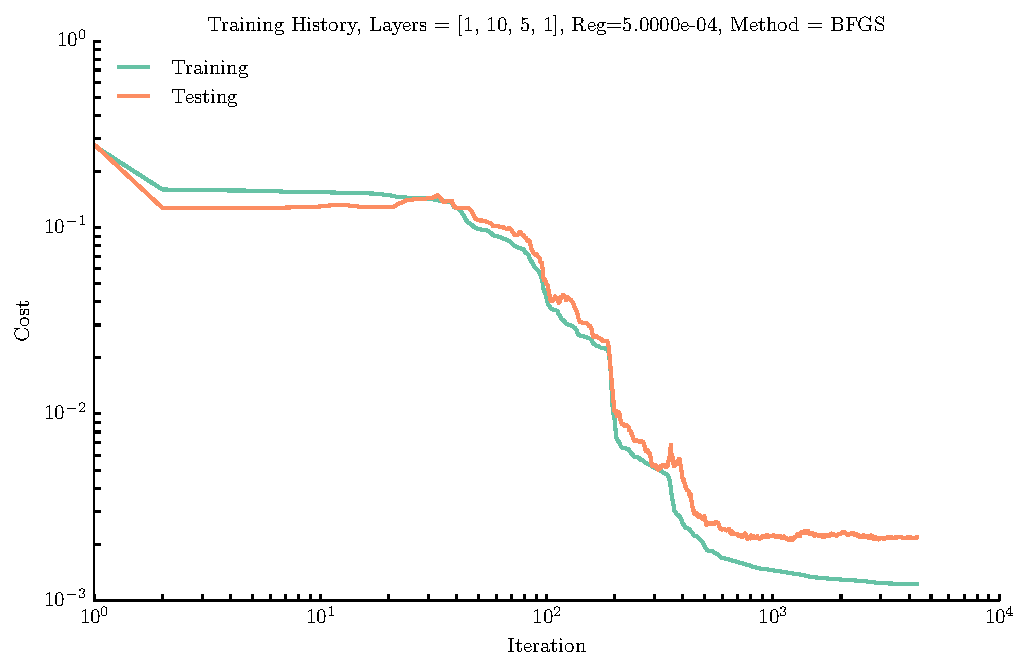
\includegraphics[width=\textwidth]{costs.pdf}
\caption{Plots of the cost function during the training of the FFNN. Note the minimal over-fitting illustrated by the testing cost curve.}
\label{fig:costReg}
\end{figure}
\begin{figure}[!htb]
\centering
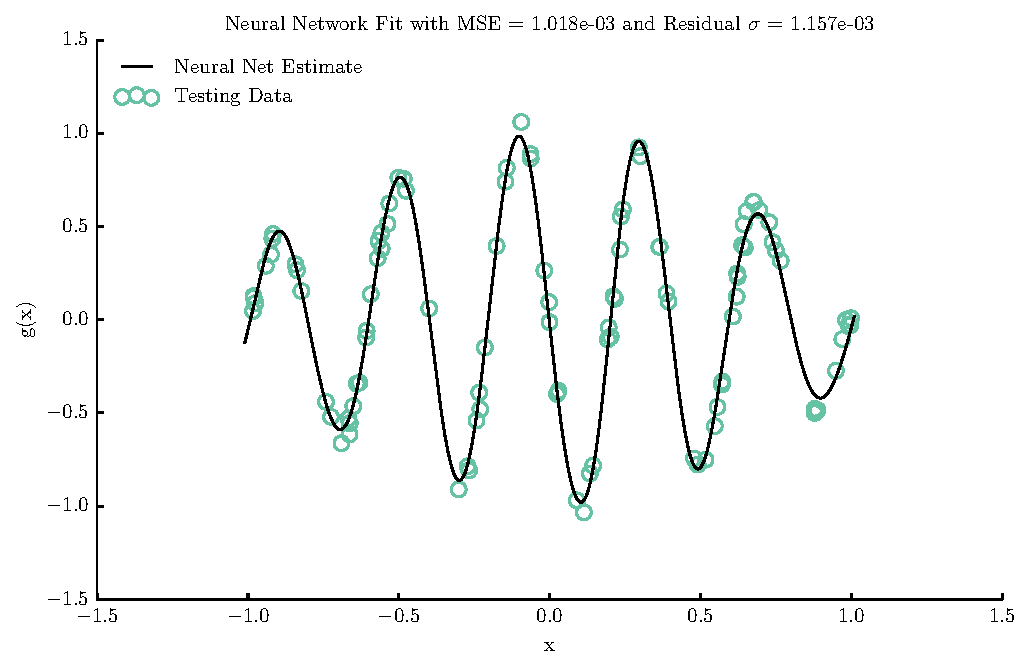
\includegraphics[width=\textwidth]{nnReg.pdf}
\caption{The neural network fit of equation \ref{g}.}
\label{fig:nnReg}
\end{figure}
\begin{figure}[!htb]
\centering
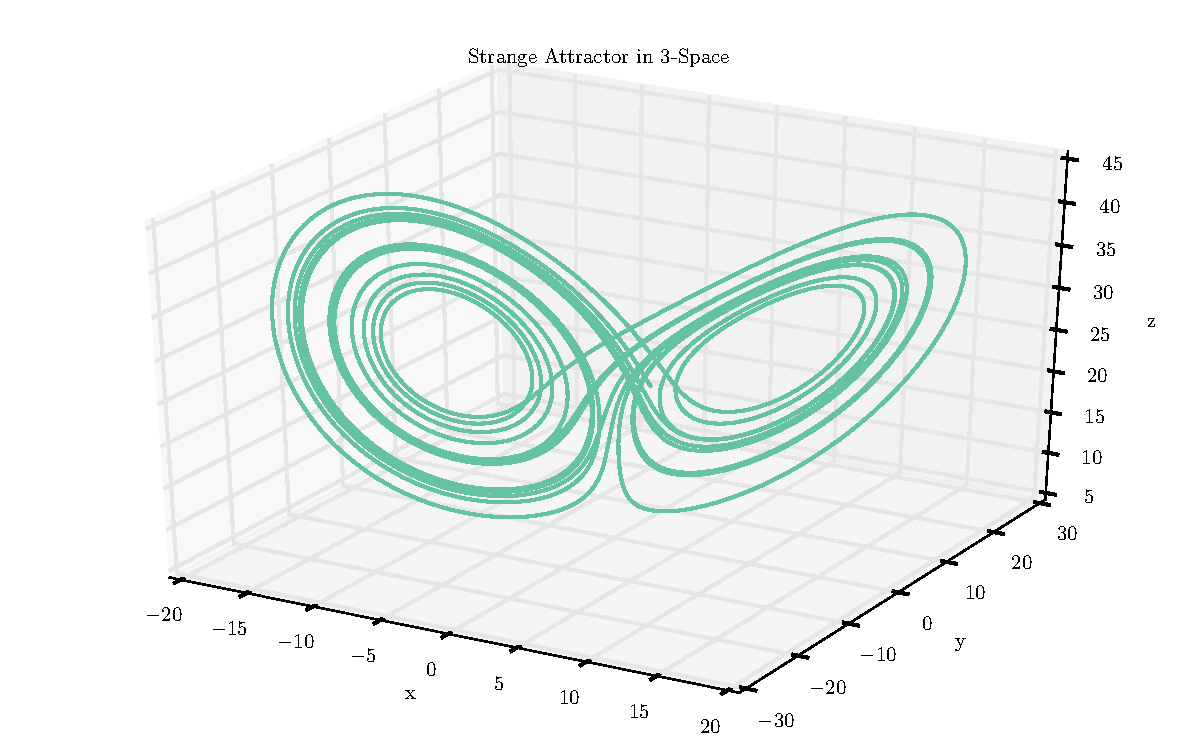
\includegraphics[width=\textwidth]{3dLorentz.pdf}
\caption{The strange attractor solution to the Lorentz system.}
\label{fig:3d Lorentz}
\end{figure}
\begin{figure}[!htb]
\centering
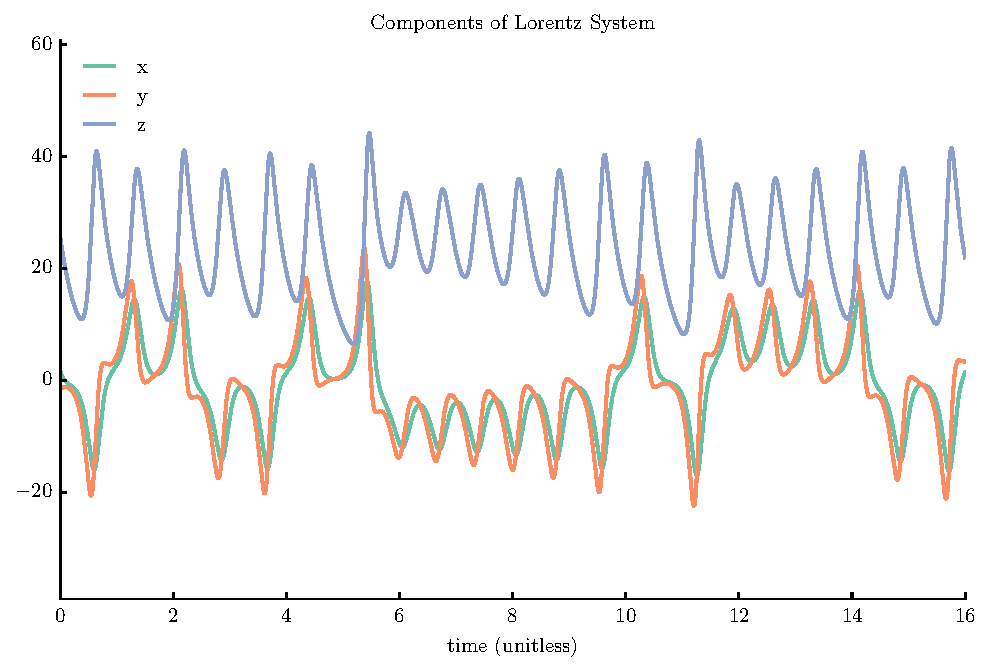
\includegraphics[width=\textwidth]{2dLorentz.pdf}
\caption{The individual components for the strange attractor solution. There is a unique multi-modal structure in which the solution persists between the two modes.}
\label{fig:2d Lorentz}
\end{figure}
\begin{figure}[!htb]
\centering
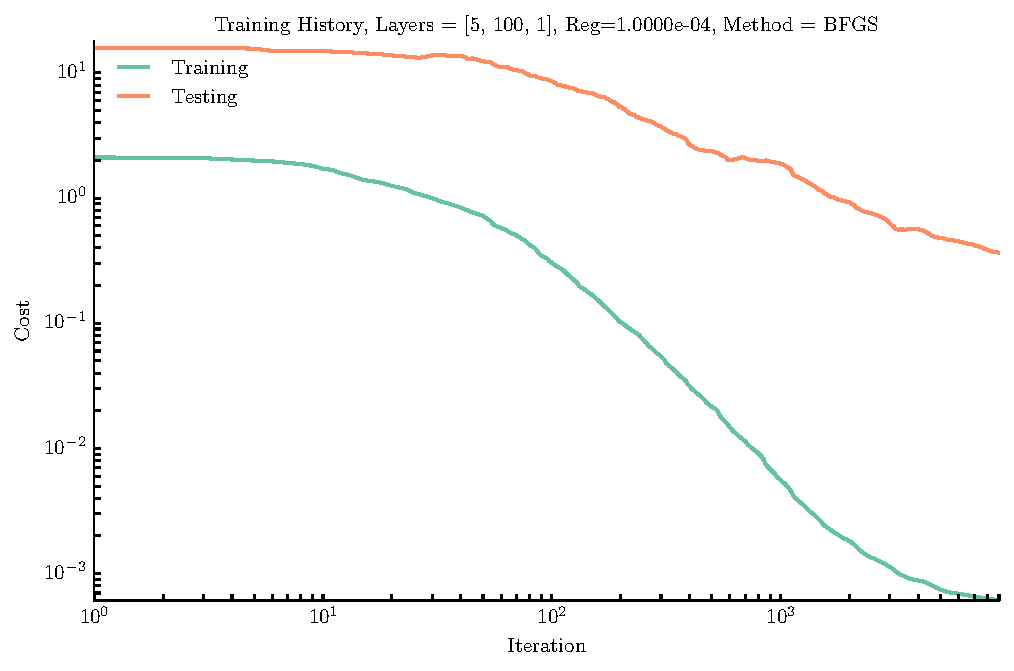
\includegraphics[width=\textwidth]{costsLorentz.pdf}
\caption{The cost function history for training the Lorentz network. The minimal over-error near the end is relatively negligible.}
\label{fig:costs Lorentz}
\end{figure}
\begin{figure}[!htb]
\centering
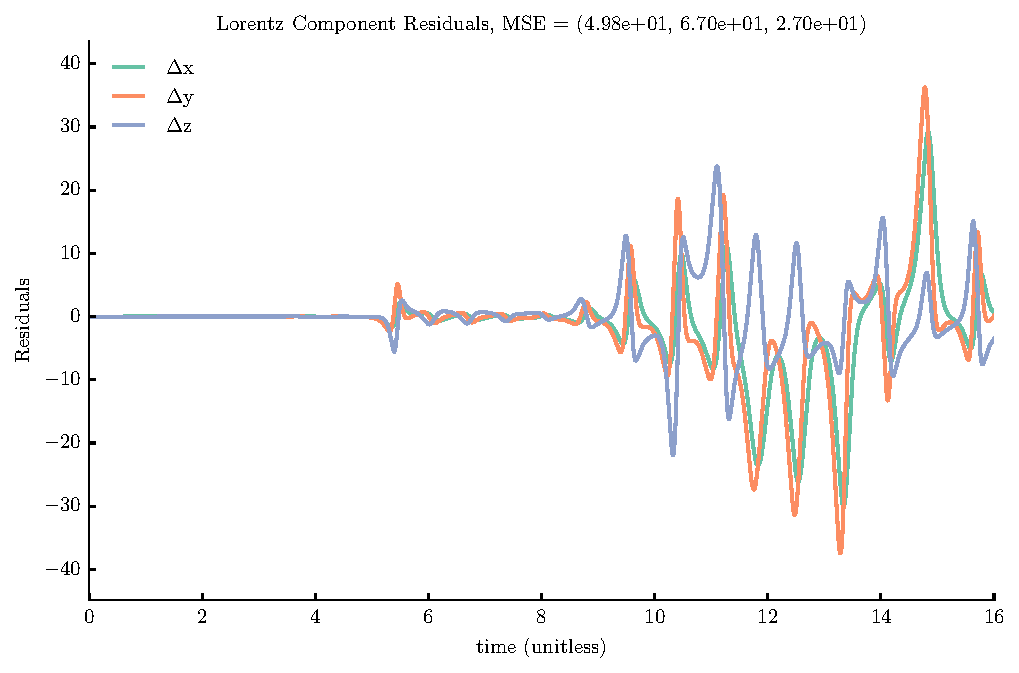
\includegraphics[width=\textwidth]{lorentz_solution.pdf}
\caption{The residuals between the trained network and the true dynamical state of the Lorentz system. The network has a good fit until the mode changes, where it loses track of the solution and errors start to accumulate quickly.}
\label{fig:nn Lorentz}
\end{figure}
\chapter{Modeling CO Fields with Neural Networks}
\label{nnco}
\section{Input Data}

The GEOS-Chem CTM was used to generate CO and atmospheric data covering a span of two years from 2006 to 2008. The model has a resolution of 4 degrees by 5 degrees and 47 vertical levels from the surface to 0.01 hPa. However, we only use data from the middle and lower troposphere (up to level 29), which have been archived hourly. The attributes selected were: day of the year, surface CO emissions, CO concentrations, wind speeds, temperature, humidity, surface pressures, and planetary boundary layer (PBL) heights. Data was restricted to a two-gridbox (8 by 5 degree) area over the New York City region to isolate mainly anthropogenic sources of CO emissions. Each of the attributes were averaged over this area and the first 17 vertical levels to reduce the dimensionality of the problem. Each attribute was standardized by its mean and variance to remove large scale differences between the data streams.

\section{Network Setup}

The FFNN was setup to ingest a time-attribute array of data and output a time-target array of CO fields. After testing with multiple layer structures, a single hidden layer with eight neurons was selected as the best model. Including more neurons returned diminishingly smaller improvements to the model, suggesting that more preprocessing work is to be done to extract features and reduce the number of degrees of freedom for this problem. Many hidden layers  also lead to similar negligible improvements, with significantly longer training times. L2 regularization was imposed on the network with a regularization coefficient of $1.00\times10^{-3}$ to reduce possible over-fitting of the training data. The network was trained for data over 2006 and tested with data over 2007 to capture seasonal structures within the attributes. 

\section{Results}

A cost analysis for the eight neuron architecture is shown in Figure \ref{fig:costCF}. The trained network has a good level of generalization, as seen from trajectory of cost cost curves. This is due to the relatively low complexity of the parameter space (81 parameters). Fitting results are summarized in Figures \ref{fig:nncoR} and \ref{fig:nncoH}. The residuals are normally distributed, indicating the FFNN captured most of the useful information and did not over-fit the testing set by assimilating the noise. The errors correlate to changes in season, but stay within approximately 12.7$\%$ of the mean CO field. Although these results indicate that smaller architectures have higher accuracy, larger networks are necessarily harder to train. Therefore, different training conditions may have to be imposed on different architectures to truly make meaningful comparisons between the different models. These networks were trained in serial on a personal computer, parallelization of the code and longer training times will likely lead to increases in prediction capabilities. All residuals were smoothed with windows of 7 days to show larger scale structure in the fit. The challenge still remains to fit the minute details in hourly variability. Figures \ref{fig:nnco28} and \ref{fig:nnco1} compare two different smoothing windows, one for 28 days and another for 1 day. The large window shows that seasonal variability is captured by the network and furthermore, that accuracy is shared between all the architectures. Note that the spread of the data is larger for the smaller window, illuminating the problem of over-fitting. Large networks need to be trained more for the same level of generalization, and In this case all three networks were trained in similar settings. Therefore, we notice a higher magnitude of noise in the fit as the number of weights increases. The raw fit without smoothing is plotted in Figure \ref{fig:nn}. There is a length of time during the summer months where the network has particular trouble fitting the small scale structure of the field. This has been a common occurrence throughout the different network architectures and will be a focus of future work on this project.
\begin{figure}[!htb]
\centering
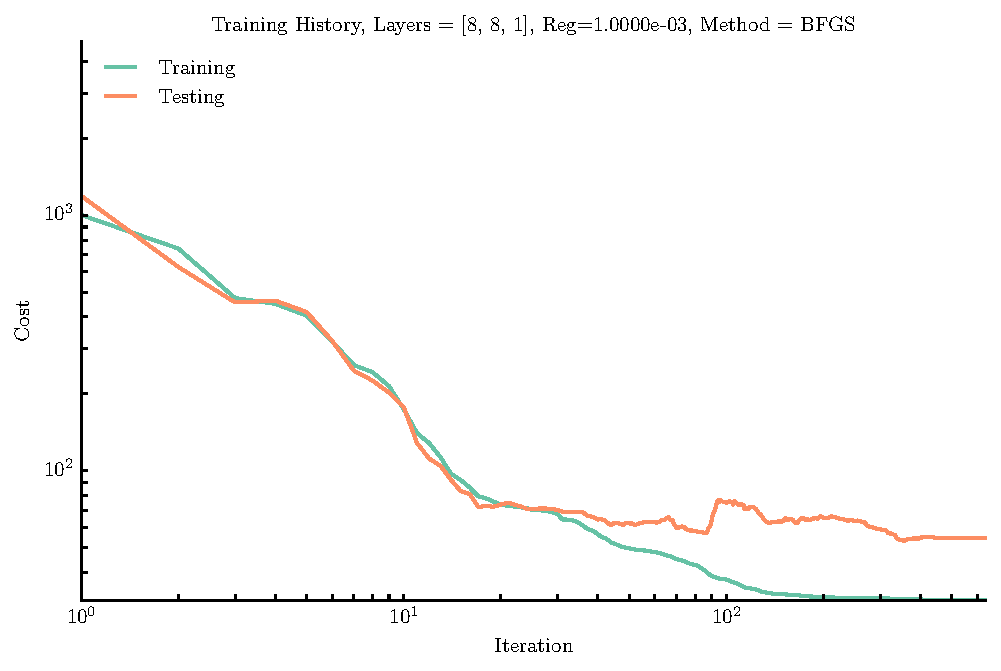
\includegraphics[width=\textwidth]{costsnnco.pdf}
\caption{The cost function history for training a FFNN on the GEOS-Chem CTM data.}
\label{fig:costCF}
\end{figure}

\begin{figure}[!htb]
\centering
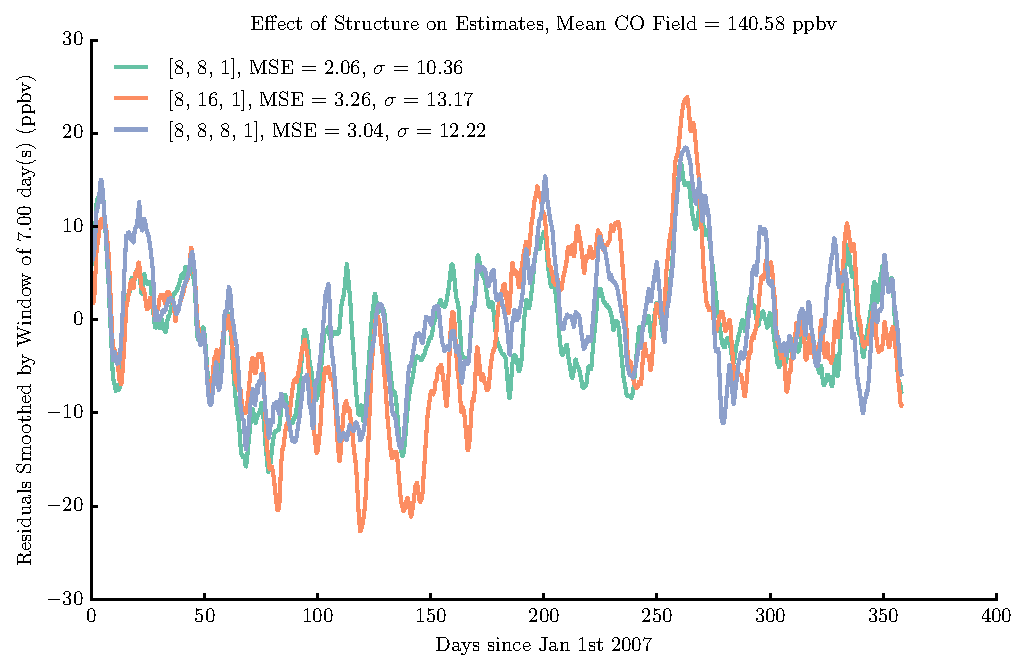
\includegraphics[width=\textwidth]{residuals_window_168.pdf}
\caption{A plot of residual data between the GEOS model and multiple neural network fits. Larger architectures do not necessarily provide proportionate improvements to the model.}
\label{fig:nncoR}
\end{figure}

\begin{figure}[!htb]
\centering
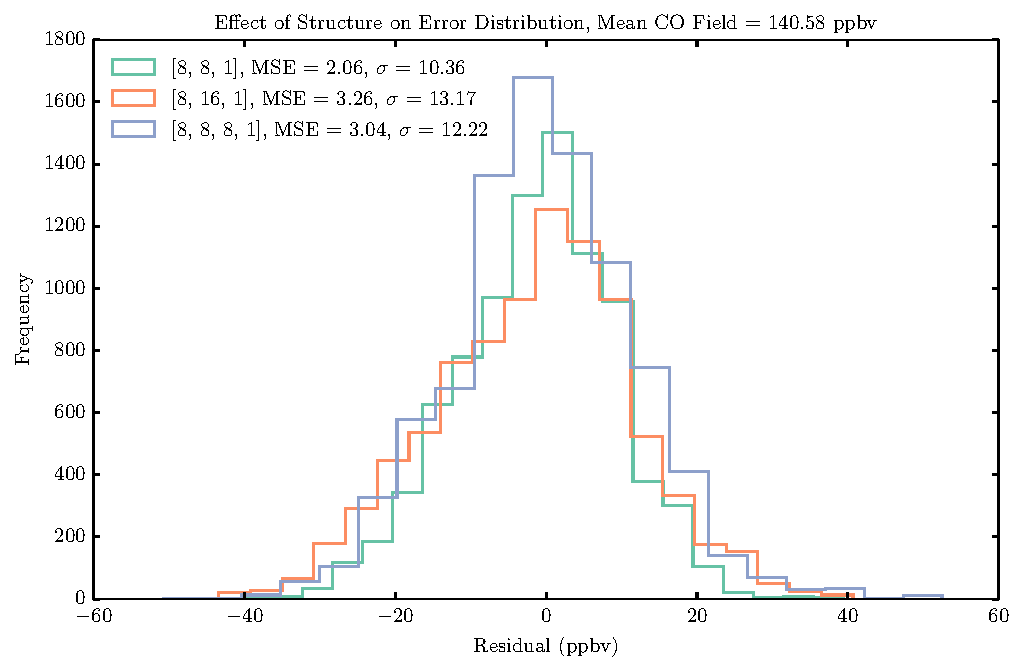
\includegraphics[width=\textwidth]{histograms.pdf}
\caption{A histogram of residuals data between the GEOS model and multiple neural network fits.}
\label{fig:nncoH}
\end{figure}

\begin{figure}[!htb]
\centering
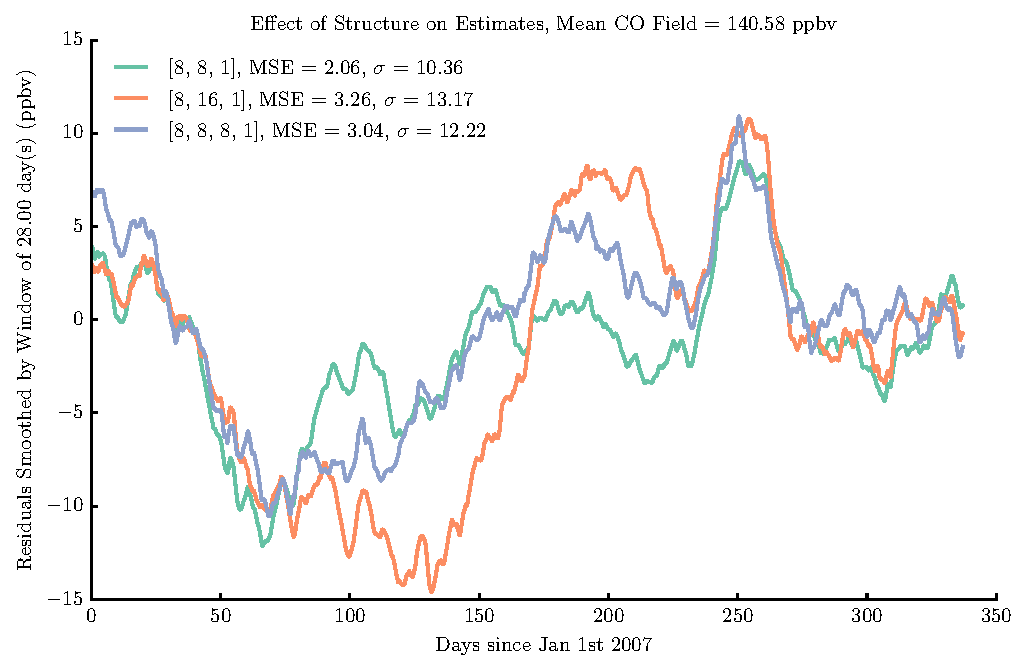
\includegraphics[width=\textwidth]{residuals_window_672.pdf}
\caption{Residuals between the GEOS-Chem CTM data and network outputs. A large smoothing window shows that all three networks capture seasonal changes without major discrepancies.}
\label{fig:nnco28}
\end{figure}

\begin{figure}[!htb]
\centering
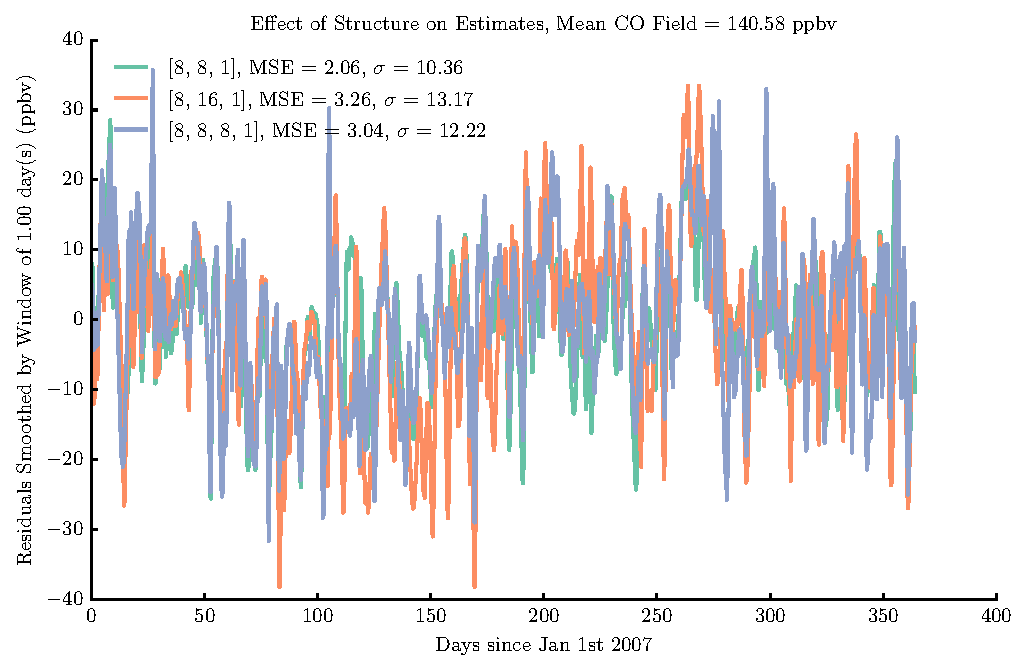
\includegraphics[width=\textwidth]{residuals_window_24.pdf}
\caption{Residuals between the GEOS-Chem CTM data and network outputs. A short smoothing window allows daily variability to leak into the data and illuminate the problem of over-fitting.}
\label{fig:nnco1}
\end{figure}

\begin{figure}[!htb]
\centering
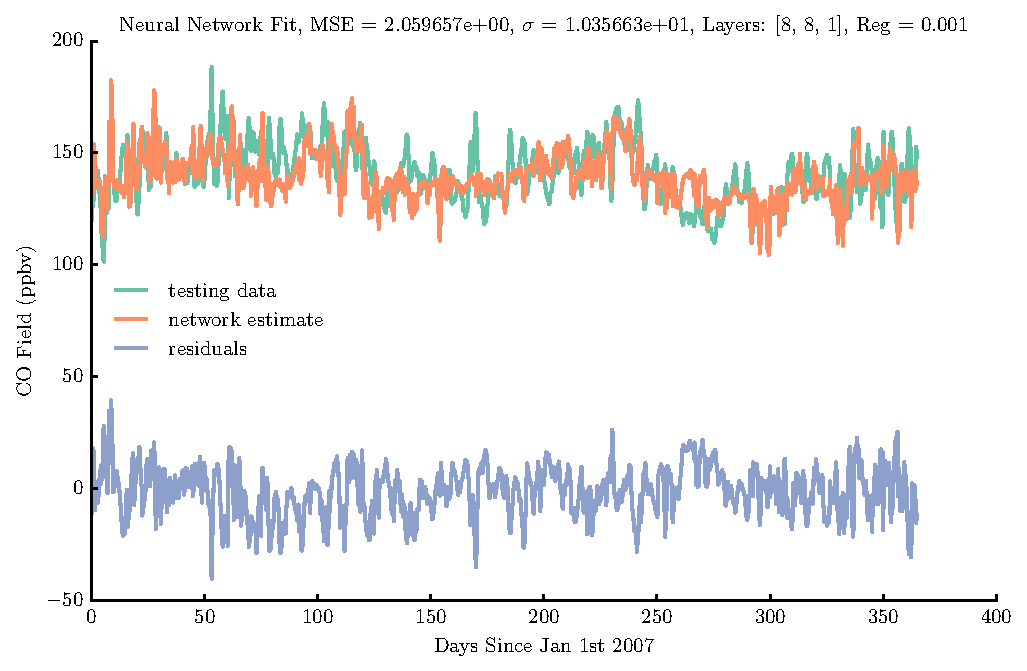
\includegraphics[width=\textwidth]{nnfield.pdf}
\caption{The raw fit of the testing data. Note the errors during the summer season.}
\label{fig:nn}
\end{figure}

\section{Conclusions and Future Work}

The statistical approach taken in these experiments have proved to be an advantageous way of modeling CO concentrations. Accurate models were constructed given short training times, small architectures, and little preprocessing of data. It is clear that given more computational resources, neural networks will be a valuable tool to use alongside modern data assimilation techniques. The next problem is one of scale. The data set is currently one dimensional in each attribute. The total GEOS-Chem CTM dataset is multivariate and of very high dimension. In order to extend this analysis to whole map modeling, efficient methods of dimension reduction must be investigated. N-way methods of tensor factorization will be considered to reduce the number of dimensions but also to retain correlation information in both spatial and temporal domains. There has been recent interest to apply convolutional neural networks to high dimensional spatial data and to use recurrent neural networks for modeling time series data. It would seem plausible then, to combine the two architectures to attack problems with both spatial and temporal correlations. Lastly, more efficient ways of training will be considered to deal with larger sets of data, as training on one year may not be enough to quantity large scale temporal activity in the data. Weight dropout, simulated annealing, and genetic algorithms will all be considered to help reach global minima in spaces that not convex and of very large size.


\addcontentsline{toc}{chapter}{Bibliography}
\bibliographystyle{apalike}
\bibliography{thebib}

\end{document}
